\documentclass{article} % For LaTeX2e
\usepackage{nips12submit_e,times}
\usepackage[latin1]{inputenc}
\usepackage{amsmath}
\usepackage{amsfonts}
\usepackage{amssymb}
\usepackage{caption} 
\usepackage{cite} 
\usepackage{subcaption} 
\usepackage[pdftex]{graphicx}
\nipsfinalcopy

\title{Saturating Auto-Encoder} 

\author{
Rostislav Goroshin \\
Courant Institute of Mathematical Science\\
New York University \\
\texttt{goroshin@cs.nyu.edu} \\
\And
Yann LeCun \\
Courant Institute of Mathematical Science\\
New York University \\
\texttt{yann@cs.nyu.edu} \\
\date{} }


\begin{document}
\maketitle

\begin{abstract} 
We introduce a simple new regularizer for auto-encoders whose hidden-unit activation functions contain at least one zero-gradient (saturated) region. This regularizer explicitly encourages activations in the saturated region(s) of the corresponding activation function. We call these Saturating Auto-Encoders (SATAE). We show that the saturation regularizer explicitly limits the SATAE's ability to reconstruct inputs which are not near the data manifold. Furthermore, we show that a wide variety of features can be learned when different activation functions are used. Finally, connections are established with the Contractive and Sparse Auto-Encoders.    

\end{abstract} 
\section{Introduction} 
An auto-encoder is a conceptually simple neural network used for obtaining useful data representations through unsupervised training. It is composed of an encoder which outputs a hidden (or latent) representation and a decoder which attempts to reconstruct the input using the hidden representation as its input. Training consists of minimizing a reconstruction cost such as $L_2$ error. However this cost is merely a proxy for the true objective: to obtain a useful latent representation. Auto-encoders can  implement many dimensionality reduction techniques such as PCA and Sparse Coding (SC) \cite{DHS}\cite{SC}\cite{LISTA}. This makes the study of auto-encoders very appealing from a theoretical standpoint. In recent years, renewed interest in auto-encoders networks has mainly been due to their empirical success in unsupervised feature learning \cite{SAE1}\cite{SAE2}\cite{CAE}\cite{DAE}. \\

\noindent
With only its reconstruction cost, the standard auto-encoder does not typically learn any meaningful hidden representation of the data. Well known theoretical and experimental results show that a linear auto-encoder with trainable encoding and decoding matrices, $W^e$ and $W^d$ respectively, learns the identity function if $W^e$ and $W^d$ are full rank or over-complete. The linear auto-encoder learns the principle variance directions (PCA) if $W^e$ and $W^d$ are rank deficient \cite{DHS}. It has been observed that other representations can be obtained by regularizing the latent representation. This approach is exemplified by the Contractive and Sparse Auto-Encoders \cite{CAE} \cite{SAE1} \cite{SAE2}. Intuitively, an auto-encoder with limited capacity will focus its resources on reconstructing portions of the input space in which data samples occur most frequently. From an energy based perspective, auto-encoders achieve low reconstruction cost in portions of the input space with high data density. If the data occupies some low dimensional manifold in the higher dimensional input space then minimizing reconstruction error achieves low energy on this manifold. Useful latent state regularizers raise the energy of points that do not lie on the manifold, thus playing an analogous role to minimizing the partition function in maximum likelihood models. In this work we introduce a new type of regularizer that does this explicitly for auto-encoders with a non-linearity that contains at least one flat (zero gradient) region. We show examples where this regularizer and the choice of nonlinearity determine the feature set that is learned by the auto-encoder.      

\section{Hidden Variable Regularization}    
Several auto-encoder variants which regularize their latent states have been proposed, they include the sparse auto-encoder and the contractive auto-encoder\cite{SAE1}\cite{SAE2}\cite{CAE}. The sparse auto-encoder includes an over-complete basis in the encoder and imposes a sparsity inducing (usually $L_1$) penalty on the hidden activations. This penalty prevents the auto-encoder from learning to reconstruct all possible points in the input space and focuses the expressive power of the auto-encoder on representing the data-manifold. Similarly, the contractive auto-encoder avoids trivial solutions by introducing an auxiliary penalty which measures the square  Frobenius norm of the Jacobian of the latent representation with respect to the inputs. This encourages a constant latent representation except around training samples where it is counteracted by the reconstruction term. It has been noted in \cite{CAE} that these two approaches are strongly related. The contractive auto-encoder explicitly encourages small entries in the Jacobian, whereas the sparse auto-encoder is encouraged to produce mostly zero (sparse) activations which can be designed to correspond to mostly flat regions of the nonlinearity, thus also yielding small entries in the Jacobian.

\subsection{Saturating Auto-Encoder through Complementary Nonlinearities}     
Our goal is to introduce a simple new regularizer which will explicitly raises reconstruction error for inputs not near the data manifold. Consider activation functions with at least one flat region; these include shrink, rectified linear, and saturated linear (Figure~\ref{fig:nonlin}). Auto-encoders with such nonlinearities lose their ability to accurately reconstruct inputs which produce activations in the saturation regime(s) of their activation functions. With this in mind, we introduce a penalty of the form $f_c(\sum_{j=1}^d W^e_{ij}x_j + b_i)$ encourages the argument to be in the saturation regime of the activation function ($f$). We call this the Saturating Auto-Encoder (SATAE). For activation functions with zero-gradient regime(s) the complementary nonlinearity ($f_c$) can be defined as the distance to the nearest saturation region. Specifically, let $S = \{x \mid  f'(x) = 0\}$ then we define $f_c(x)$ as: 

\begin{equation}
f_c(x) = \inf_ {y \in S} |x-y|.   
\end{equation}   

\begin{figure}
\centering 
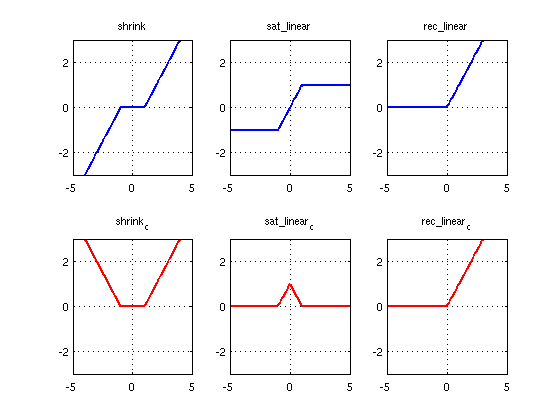
\includegraphics[scale=0.6]{compliments.png}
\caption{Three nonlinearities (top) with their associated complementary regularization functions(bottom).}  
\label{fig:nonlin}
\end{figure} 

\noindent
Figure 1 shows three activation functions and their associated complementary nonlinearities. The complete loss to be minimized by a SATAE with nonlinearity $f$ is: 

\begin{equation} 
L = \sum_{x \in D} \frac{1}{2} \|x-x_r\|^2 + \eta \sum_{i=1}^{d_h}f_c(W^e_i x + b^e_i),
\end{equation}    

\noindent
where $x_r = W^df(W^e x + b^e) + b^d$ is the reconstructed $x$ for an auto-encoder with no output nonlinearity, and $d_h$ denote the number of hidden units. The hyper-parameter $\eta$ regulates the trade-off between reconstruction and saturation.  

\section{Effect of the Saturation Regularizer} 
We will examine the effect of the saturation regularizer on auto-encoders with a variety of activation functions. It will be shown that the choice of activation function is a significant factor in determining the type of basis the SATAE learns. First, we will present results on toy data in two dimensions followed by results on higher dimensional image data. 

\subsection{Visualizing the Energy Landscape}  
Given a trained auto-encoder the reconstruction error can be evaluated for a given input $x$. For low-dimensional spaces ($\mathbb{R}^n$, where $n \leq 3$) we can evaluate the reconstruction error on a regular grid in order to visualize the portions of the space which are well represented by the auto-encoder. More specifically we can compute $E(x) = \frac{1}{2} \|x - x_r \|^2$ for all $x$ within some bounded region of the input space. Ideally, the reconstruction energy will be low for all $x$ which are in training set and high elsewhere. Figures~\ref{fig:toyshrink} and~\ref{fig:toysatlinear} depict the resulting reconstruction energy for inputs $x \in \mathbb{R}^2$, and  $-1 \leq x_i \leq 1$. Black corresponds to low reconstruction energy. The training data consists of a one dimensional manifold shown overlain in yellow. Figure~\ref{fig:toyshrink} shows a toy example for a SATAE which uses ten basis vectors and a shrink activation function. Note that adding the saturation regularizer decreases the volume of the space which is well reconstructed, however good reconstruction is maintained on or near the training data manifold. The auto-encoder in Figure~\ref{fig:toysatlinear} contains two encoding basis vectors (red), two decoding basis vectors (green), and uses a saturated-linear activation function. The encoding and decoding bases are unconstrained. The unregularized auto-encoder learns an orthogonal basis with a random orientation. The region of the space which is well reconstructed corresponds to the outer product of the linear regions of two activation functions; beyond that the error increases quadratically with the distance. Including the saturation regularizer however induces the auto-encoder to operate in the saturation regime at the extreme points of the training data, limiting the space which is well reconstructed. Note that because the encoding and decoding weights are separate and unrestricted, the encoding weights were scaled up to effectively reduce the width of the linear regime of the nonlinearity. 

\subsection{SATAE-shrink}
Consider a SATAE with a shrink activation function and shrink parameter $\lambda$. The corresponding complementary nonlinearity, derived using Equation 1 is given by: 
\begin{equation} 
\nonumber
shrink_c(x) =
\begin{cases}
abs(x), \text{ } |x| > \lambda\\
0, \text{ elsewhere}
\end{cases}.
\end{equation} 

\begin{figure}
\centering 
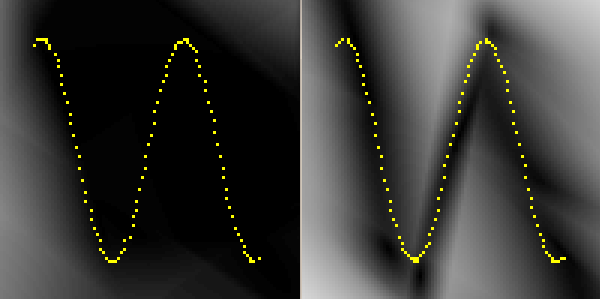
\includegraphics[scale=0.25]{toy_shrink.png}
\caption{Energy surfaces for unregularized (left), and regularized (right) solutions obtained using the $shrink$ nonlinearity and 10 basis vectors. Black corresponds to low reconstruction energy. Training points lie on a one-dimensional manifold shown in yellow.}  
\label{fig:toyshrink}
\end{figure} 

\begin{figure}
\centering 
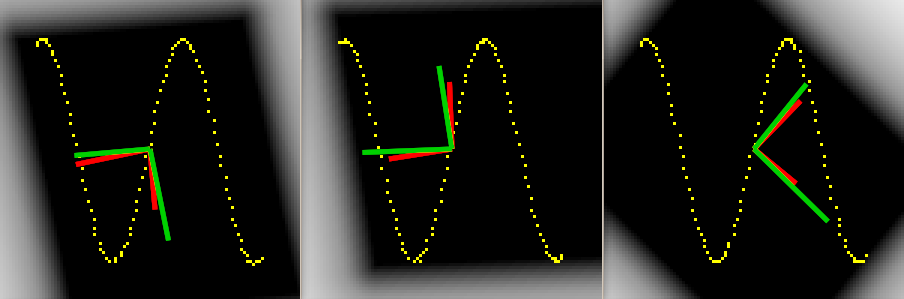
\includegraphics[scale=0.25]{toy_sat_linear_noreg.png}
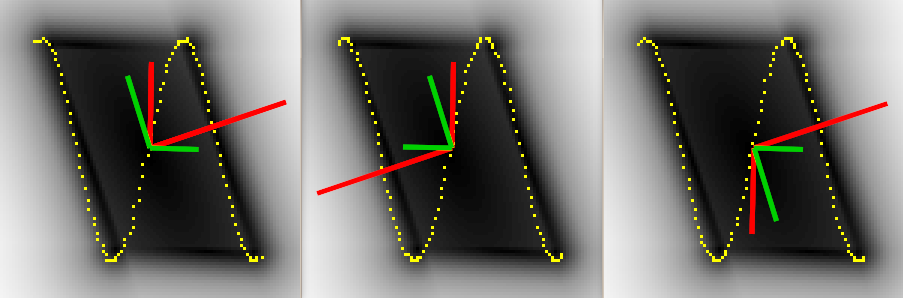
\includegraphics[scale=0.25]{toy_sat_linear_reg.png}
\caption{Top Row: three randomly initialized solutions obtained with no regularization. Bottom Row: three randomly initialized solutions obtained with regularization.}  
\label{fig:toysatlinear} 
\end{figure} 

Note that $shrink_c(W^e x + b^e) =  abs(shrink(W^e x + b^e))$, which corresponds to an $L_1$ penalty on the activations. Thus this SATAE is equivalent to a sparse auto-encoder with a shrink activation function. Given the equivalence to the sparse auto-encoder we anticipate the same scale ambiguity which occurs with $L_1$ regularization. This ambiguity can be avoided by normalizing the decoder weights to unit norm. It is expected that the SATAE-shrink will learn similar features to those obtain with a sparse auto-encoder, and indeed this is what we observe. Figure~\ref{fig:patches}(a) shows 25 randomly selected decoder filters learned by an auto-encoder with shrink nonlinearity trained on natural 12x12 image patches. One can recognize the expected Gabor-like features when the saturation penalty is activated. When trained on the binary MNIST dataset the learned basis is comprised of portions of digits and strokes. Nearly identical results are obtained with a SATAE which uses a rectified-linear activation function. This is because a rectified-linear function with a bias can behave like as a positive only shrink function, similarly the complementary function is equivalent to a positive only $L_1$ penalty on the activations.          

\begin{figure}
\centering
	\begin{subfigure}[b]{0.2\textwidth}
		\centering 
		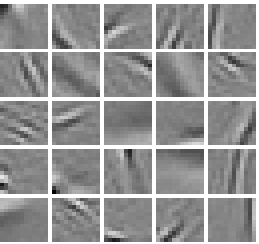
\includegraphics[scale=0.3]{shrink_reg_and_norm.png}
		\caption{}
	\end{subfigure} 
	\begin{subfigure}[b]{0.2\textwidth}
		\centering 
		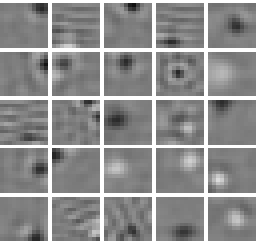
\includegraphics[scale=0.3]{sat_linear_reg2.png}
		\caption{}
	\end{subfigure} 
\caption{(a)Twenty-five randomly selected basis elements learned by the SATAE with shrink nonlinearity trained on 12x12 natural image patches. (b) Identical to (a), except that the SATAE uses a saturated-linear nonlinearity}
\label{fig:patches}
\end{figure} 

\begin{figure}
\centering 
\begin{subfigure}[b]{0.225\textwidth}
		\centering 
		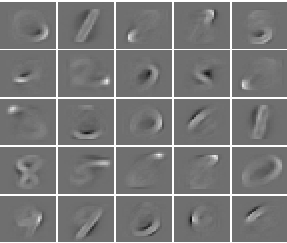
\includegraphics[scale=0.3]{strokes.png}
		\caption{}
	\end{subfigure} 
	\begin{subfigure}[b]{0.225\textwidth}
		\centering 
		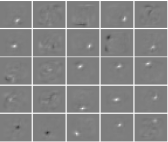
\includegraphics[scale=0.515]{ident.png}
		\caption{}
	\end{subfigure} 
\caption{(a)Twenty-five randomly selected basis elements learned by the SATAE with shrink nonlinearity trained on 28x28 binary MNIST digits. (b) Identical to (a), except that the SATAE uses a saturated-linear nonlinearity}
\label{fig:MNIST}
\end{figure} 

\subsection{SATAE-saturated-linear} 
The SATAE with saturated-linear activation function learns a completely different feature set. Empirically, it was observed that increasing the regularization penalty produces more localized feature detectors. To understand why these feature detectors arise consider a dataset in which the variables take on binary values (e.g. MNIST). The scaled identity basis is a global minimizer of Equation 2 when a saturated-linear activation function is used. Such a basis can perfectly reconstruct any binary input while operating exclusively in the saturated regions of the activation function, thus incurring no saturation penalty. This is exactly the type of basis that arises in experiments when training on MNIST, see Figure~\ref{fig:MNIST}b. Training on image patches produces a similar but less pronounced effect: more localized features are obtained but of greater variety (Figure~\ref{fig:patches}b). In contrast to the SATAE-shrink, the SATAE-saturated-linear receives the heaviest penalty when the activation is zero, which tends to spread the responsibility of reconstructing the data among all the basis elements.   

\section{Experimental Details}
In all experiments data samples were normalized by subtracting the mean and dividing by the standard deviation of the dataset. Experiments on MNIST were performed with 200 basis elements, while experiments on natural image patches used only 100 basis elements. The decoder basis elements of the SATAEs with shrink and rectified-linear nonlinearities were reprojected to the unit sphere after every 10 stochastic gradient updates. The SATAEs which used saturated-linear activation function were trained with tied weights. All results presented were obtained using stochastic gradient descent.

\section{Discussion}
We have demonstrated that by using different activation functions drastically different feature sets are learned by SATAEs. Hybrid SATAEs which use a mixture of activation functions also possible. The utility of these features depend on the application.  

\subsection{Relationship with the Contractive Auto-Encoder} 
Let $h_i$ be the output of the $i^{th}$ hidden unit of a single-layer auto-encoder with point-wise nonlinearity $f(\cdot)$. The regularizer imposed by the contractive auto-encoder (CAE) can be expressed as follows: 

\begin{equation}
\nonumber
\sum_{ij} \left(\frac{\partial h_i}{\partial x_j} \right)^2 = \sum_i ^{d_h} \left(f'(\sum_{j=1}^d W^e_{ij}x_j + b_i)^2 \| W^e_i \| ^2 \right),
\end{equation}  
 
\noindent
where $x$ is a $d$-dimensional data vector, $f'(\cdot)$ is the derivative of $f(\cdot)$, $b_i$ is the bias of the $i^{th}$ encoding unit, and $W^e_i$ denotes the $i^{th}$ row of the encoding weight matrix. The first term in the above equation tries to adjust the weights so as to push the activations into the low gradient (saturation) regime of the nonlinearity, but is only defined for differentiable activation functions. Therefore the CAE indirectly encourages operation in the saturation regime. Computing the Jacobian, however, can be cumbersome for deep networks. Furthermore, the complexity of computing the Jacobian is $O(d \times d_h)$ \cite{CAE}, compared to the $O(d_h)$ for the saturation penalty.  

 
\subsection{Relationship with the Sparse Auto-Encoder}

In Section 3.2 it was shown that SATAEs with shrink or rectified-linear activation functions are equivalent to a sparse auto-encoder. Like the sparsity penalty, the saturation penalty can be applied at any point in a deep network at the same computational cost. Unlike the sparsity penalty, the saturation penalty is adapted to the nonlinearity of the particular layer to which it is applied. 
 
 \begin{thebibliography}{1}

\bibitem{SAE1} Marc'Aurelio Ranzato, Christopher Poultney, Sumit Chopra and Yann LeCun. Efficient Learning of Sparse Representations with an Energy-	   Based Model, in J. Platt et al. (Eds), {\em Advances in Neural Information Processing Systems (NIPS 2006)}, 19, MIT Press, 2006.

\bibitem{SAE2} Marc'Aurelio Ranzato, Fu-Jie Huang, Y-Lan Boureau and Yann LeCun: Unsupervised Learning of Invariant Feature Hierarchies with Applications to Object Recognition, Proc. {\em Computer Vision and Pattern Recognition Conference (CVPR'07)}, IEEE Press, 2007
 
\bibitem{CAE} Rifai, S. and Vincent, P. and Muller, X. and Glorot, X. and Bengio, Y. Contractive auto-encoders: Explicit invariance during feature extraction, {\em Proceedings of the Twenty-eight International Conference on Machine Learning,  ICML 2011}

\bibitem{DAE} P. Vincent, H. Larochelle, Y. Bengio, P.A. Manzagol. Extracting and Composing Robust Features with Denoising Autoencoders
{\em Proceedings of the 25th International Conference on Machine Learning (ICML'2008)}, 2008.

\bibitem{DHS} R.O. Duda, P.E. Hart, and D.G. Stork, Pattern Classification, New York: John Wiley \& Sons, 2001, pp. xx + 654, ISBN: 0-471-05669-3

\bibitem{SC} Olhausen, Bruno A.; Field, David J. (1997). Sparse Coding with an Overcomplete Basis Set: A Strategy Employed by V1?. {\em Vision Research 37 (23): 3311-3325.}

\bibitem{LISTA} Karol Gregor and Yann LeCun: Learning Fast Approximations of Sparse Coding, Proc. {\em International Conference on Machine learning (ICML'10)}, 2010

\end{thebibliography}

\end{document} 








